

In our experiments, we first demonstrate the fundamental limitations of existing discussion-based orchestration methods when applied to SLMs (Section~\ref{sec:comparison}). We then evaluate the proposed \NAME{} in Section~\ref{sub:vanilla}. In Section~\ref{sub:search-results}, we access our proposed search strategy. Finally, in Section~\ref{sub:scaling-results}, we examine the compute scaling strategies.
% We design a comprehensive experimental setup across multiple datasets and model scales to rigorously assess these questions.

\vspace{3pt}
\subsection{Existing Discussion-Based Orchestration Methods Harm SLM Performance}
\vspace{3pt}
\label{sec:comparison}

% We evaluate three discussion-based composition architectures: LLM-Debate~\citep{du2023improvingfactualityreasoninglanguage}, Mixture-of-Agents~\citep{wang2024mixtureofagentsenhanceslargelanguage}, and Multi-Agent Verification~\citep{lifshitz2025multiagentverificationscalingtesttime}. We use the same experimental settings for SLMs and frontier LLMs; we vary only the choice of models between a small-sized group and a frontier (often larger) group.

To understand whether orchestration methods developed for frontier LLMs are suitable for SLMs, we conduct a systematic comparison across model scales. We evaluate three prominent discussion-based methods—LLM-Debate~\citep{du2023improvingfactualityreasoninglanguage}, Mixture-of-Agents~\citep{wang2024mixtureofagentsenhanceslargelanguage}, and Multi-Agent Verification~\citep{lifshitz2025multiagentverificationscalingtesttime} —using identical experimental settings on both SLMs (Llama 3.1 8B~\citep{jiang2024mixtralexperts}, Mistral 8×7B~\citep{grattafiori2024llama3herdmodels}, Gemma 2 27B) and frontier LLMs (DeepSeek V3~\citep{deepseekai2025deepseekv3technicalreport}, Gemini 2.0 Flash~\citep{google2025gemini2flash}, GPT-4o~\citep{openai2024gpt4ocard}). Evaluation is conducted on MATH and GPQA datasets using original implementations and prompts.


\paragraph{Results} As shown in Figure~\ref{fig:small-large-accuracy}, discussion-based methods generally outperform the single best-performing models in the frontier LLM group, achieving up to a 2\% increase in accuracy. However, when applied to SLMs, these discussion-based methods fail to outperform the best single model in the orchestration, and even incur accuracy drops of up to 5.5\%. This performance gap is observed across all three methods and both benchmarks. 

To understand this counterintuitive result, we analyze SLM behavior in discussion settings. We find that discussion-based methods amplify rather than correct errors in SLMs due to a key limitations: SLMs tend to exhibit groupthink, reinforcing incorrect reasoning during discussions rather than correcting mistakes. Additional analysis and demonstration is provided in the Appendix~\ref{sec:slm-failure}.



\begin{figure}[htbp]
  \centering
  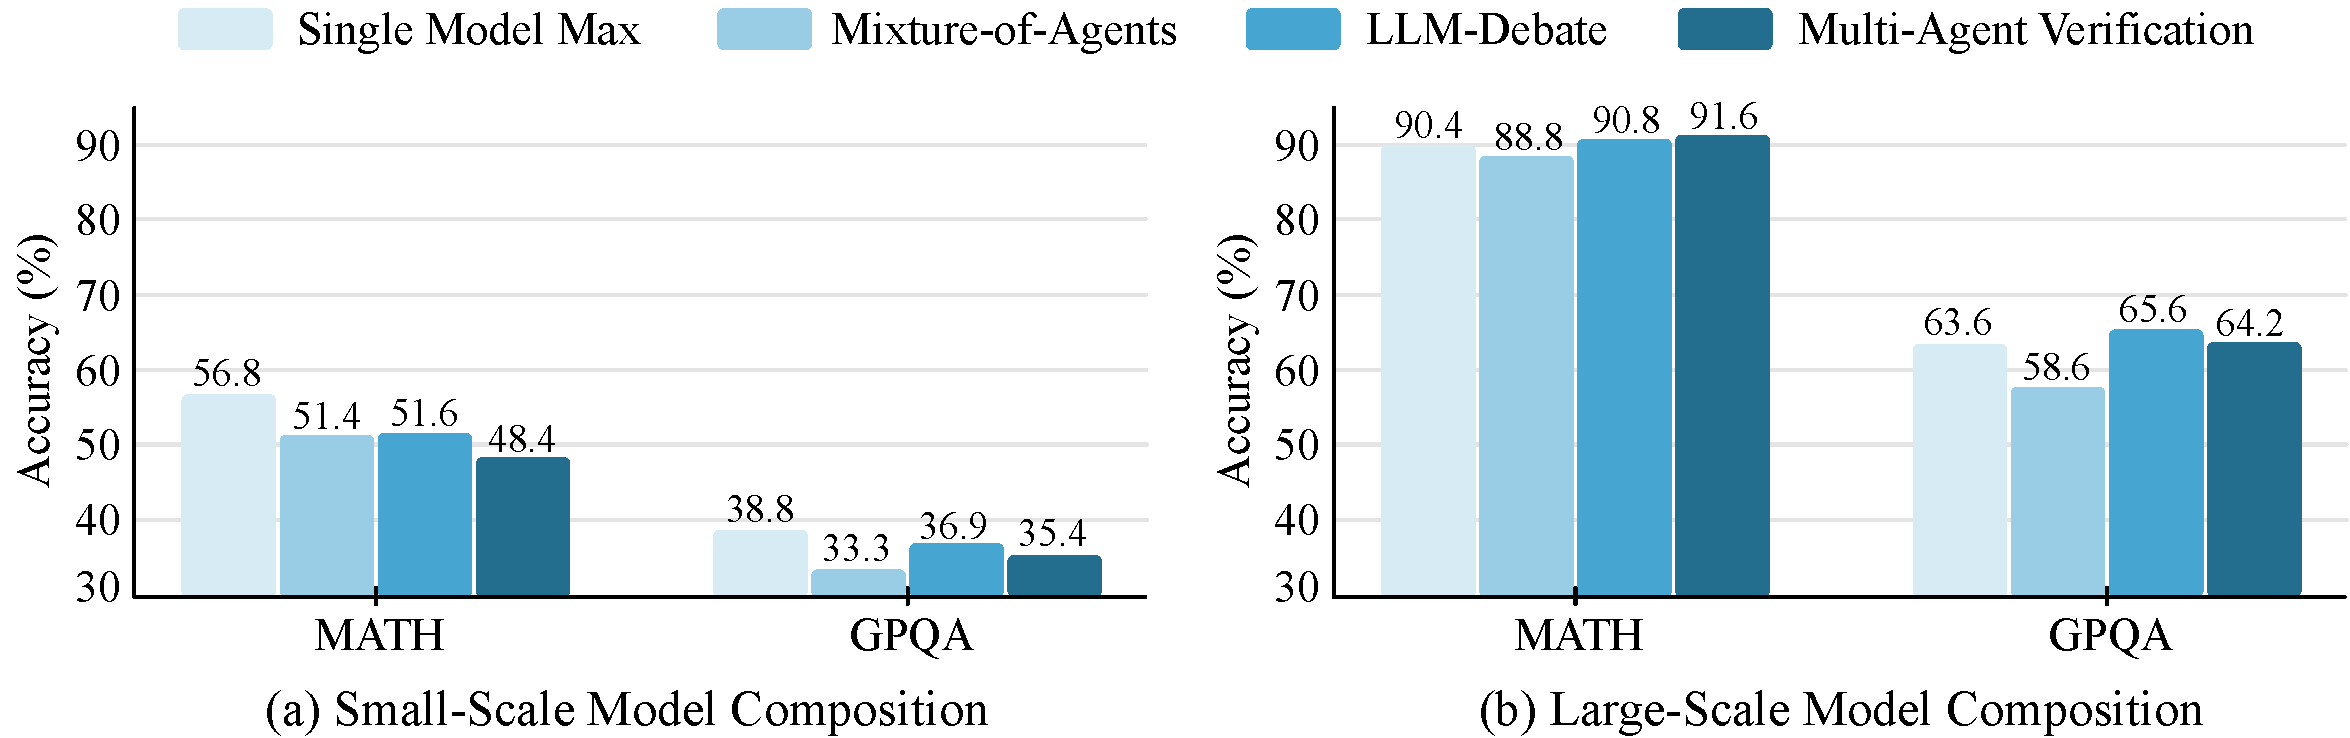
\includegraphics[width=0.9\linewidth]{Figures/Small-large-acc-light-blue_v2.pdf}
  \vspace{-8pt}
  \caption{\small \textbf{Comparison of discussion-based orchestration when invoking SLMs and LLMs.} We compare three orchestration methods (Mixture-of-Agents, LLM-Debate, and Verification) using (a) SLMs (Llama 3.1 8B, Mistral 8$\times$7B, Gemma 2 27B) and (b) frontier LLMs (DeepSeek V3, Gemini 2.0 Flash, GPT-4o) on the \textsc{MATH} and \textsc{GPQA} datasets. The baseline (\textit{Single-Model Max}) reflects the best performance of individual models. A orchestration is considered successful if it surpasses Single-Model Max.}\label{fig:small-large-accuracy}
  \vspace{-10pt}
\end{figure}



\vspace{3pt}
\subsection{\NAME{} Achieves SLM Orchestration Where Existing Methods Fail}
\vspace{3pt}
\label{sub:vanilla}

\begin{wrapfigure}{r}{0.4\textwidth}
    \centering
    \vspace{-20pt}
    \includegraphics[width=.85\linewidth]{Figures/math_distribution_pie.pdf}
    \caption{\textbf{Final Output Attribution}. We report the percentage of outputs contributed by each model on the MATH dataset for our \NAME{}. These results are from the same run as in Table~\ref{tab:composition-combined}.}
    \label{fig:output_percentage_math}
    \vspace{-5pt}
\end{wrapfigure}

To evaluate whether our proposed \NAME{} can successfully orchestrate SLMs, we test it against the same baselines from Section~\ref{sec:comparison}.  We use Mistral 8$\times$7B, LLaMA 3.1 8B, and Gemma 2 27B~\citep{gemmateam2024gemma2improvingopen} as base models. We implement the \NAME{} as follows. First, we generate three rounds of answers with a temperature of 0.3. Next, we compute a confidence score by counting how often the most common answer appears across these rounds. The final answer for each model is chosen as the most frequent one; in the case of a tie, we select the answer from the model with the highest validation accuracy. We evaluate three types of baselines. First, we measure the accuracies of individual models and report the best-performing ones. Next, for comparison with existing discussion-based methods, we include LLM-Debate~\citep{du2023improvingfactualityreasoninglanguage}, Mixture-of-Agents~\citep{wang2024mixtureofagentsenhanceslargelanguage}, and Multi-Agent Verification~\citep{lifshitz2025multiagentverificationscalingtesttime}. We follow the original workflow designs and prompts described in their papers. Experiments are conducted on three benchmark datasets: MATH~\citep{hendrycks2021measuringmathematicalproblemsolving}, GPQA~\citep{rein2023gpqagraduatelevelgoogleproofqa}, and GSM8K~\citep{cobbe2021trainingverifierssolvemath}. 




% \begin{figure}[hbtp]
%     \centering
%     \includegraphics[width=\textwidth]{iclr2026/Figures/math_distribution_pie.pdf}
%     \vspace{-20pt}
%     \caption{\textbf{Final Output Attribution}. We report the percentage of outputs contributed by each model on the MATH dataset for our \NAME{}. These results are from the same run as in Table~\ref{tab:composition-combined}. }
%     \vspace{-10pt}
%     \label{fig:output_percentage_math}
% \end{figure}


\looseness=-1
\paragraph{Results} Table~\ref{tab:composition-combined} summarizes the results. In our experiments, we find that for SLMs, existing orchestration methods do not consistently outperform the strongest individual base models or self-consistency approaches. In contrast, our \NAME{} generally achieves an accuracy gain. Compared with other approaches, our method yields up to a 13.4\% improvement on MATH, up to 8.8\% on GPQA, and up to 7.0\% on GSM8K.  These results demonstrate that the \NAME{} itself provides a clear advantage over alternative orchestration approaches at the architectural level. 

To better illustrate our proposed \NAME{}, we plot the output attribution for the MATH experiment (Table~\ref{tab:composition-combined}) in Figure~\ref{fig:output_percentage_math}. By selecting diverse outputs from the generation, \NAME{} leverages the complementary strengths of different SLMs.




% % -------- Table 2: Composition Results --------
% \begin{table}[t]
% \centering
% \small
% \begin{tabular}{lccc}
% \toprule
% \textbf{Method} & \textbf{MATH Acc (\%)} & \textbf{GPQA Acc (\%)} & \textbf{GSM8K Acc (\%)} \\
% \midrule
% Mixture-of-Agents          & 51.4 & 33.3 & 81.6 \\
% LLM-Debate                  & 51.6 & 36.8 & 80.8 \\
% Multi-Agent Verification    & 48.4 & 35.3 & 86.4 \\
% \textbf{\NAME{} (Ours)}         & \textbf{$63.0 \pm 2.16$} & \textbf{$41.9 \pm 3.52$ } & \textbf{$88.4 \pm 1.43$} \\
% \midrule
% Single-Best                 & 56.8 & 38.9 & 84.2 \\
% Single-Best-SC                 & $58.0 \pm 2.21$ & $42.4 \pm 3.53$ & $86.8 \pm 1.51$ \\
% Upper Bound                 & 64.6 & 57.0 & 92.0 \\
% \bottomrule
% \end{tabular}
% \vspace{-5pt}
% \caption{\small \textbf{\NAME{} Improves Reasoning Performance.} Accuracy of orchestration methods on MATH, GPQA, and GSM8K.}
% \label{tab:composition-combined}
% \vspace{-5pt}
% \end{table}

\begin{table}[ht]
\centering
\setlength{\tabcolsep}{15pt}
\renewcommand{\arraystretch}{0.9}
\resizebox{\textwidth}{!}{
\small
\vspace{-5pt}
\begin{tabular}{lccc}
\toprule
\textbf{Method} & \textbf{MATH Acc (\%)} & \textbf{GPQA Acc (\%)} & \textbf{GSM8K Acc (\%)} \\
\midrule
Mixture-of-Agents          & 51.4 $\pm$ 2.2 & 33.3 $\pm$ 3.4 & 81.6 $\pm$ 1.7 \\
LLM-Debate                 & 51.6 $\pm$ 2.2 & 36.8 $\pm$ 3.4 & 80.8 $\pm$ 1.8 \\
Multi-Agent Verification   & 48.4 $\pm$ 2.2 & 35.3 $\pm$ 3.4 & 86.4 $\pm$ 1.5 \\
\textbf{\NAME{} (Ours)}    & \textbf{61.8 $\pm$ 1.2} & 42.1 $\pm$ 0.3 & \textbf{87.8 $\pm$ 0.6} \\
\midrule
Single-Best                & 56.8 $\pm$ 2.2 & 38.9 $\pm$ 3.5 & 84.2 $\pm$ 1.6 \\
Single-Best-SC             & 58.0 $\pm$ 2.2 & \textbf{42.4 $\pm$ 3.5} & 86.8 $\pm$ 1.5 \\
% Upper Bound                & 64.6 $\pm$ 2.14 & 57.0 $\pm$ 3.54 & 92.0 $\pm$ 1.21 \\
\bottomrule
\end{tabular}
}
\vspace{-5pt}
\caption{\small \textbf{Accuracy with Standard Error.} The standard error across MATH, GPQA, and GSM8K for various methods. }
\label{tab:composition-combined}
\vspace{-5pt}
\end{table}




% Please ensure you have these two packages in your preamble (after \documentclass{...})
% \usepackage{tabularx}
% \usepackage{array}

% \begin{table}[t]
% \centering
% \small
% % Corrected a typo in the caption (founded -> found)
% \caption{\small \textbf{Model Combination Search results} Best model combinations found for different datasets and objectives across varying numbers of models involved (K). For clarity we just show K = 1, 2, 3 here, full results with K up to 7 can be found in appendix. }
% \label{tab:SLM-Mux-model-search-heterogeneity-adjusted}
% % Use the tabularx environment with a total width of \textwidth
% % Keep 'll' columns as is, use left-aligned, auto-adjusting X columns for the last three
% \begin{tabularx}{\textwidth}{ll >{\raggedright\arraybackslash}X >{\raggedright\arraybackslash}X >{\raggedright\arraybackslash}X}
% \toprule
% \textbf{Dataset} & \textbf{Objective} & \textbf{K=1} & \textbf{K=2} & \textbf{K=3} \\
% \midrule
% \multirow{4}{*}{\textbf{MATH}}
%  & Accuracy
%  & Qwen2.5-7B  % Abbreviated "Instruct"
%  & Mistral Small 24B  \newline Qwen2.5-7B 
%  & Gemma 2 27B \newline Mistral Small 24B  \newline Qwen2.5-7B  \\
% \cmidrule{2-5}
%  & Heterogeneity
%  & --
%  & Gemma 2 27B \newline Llama 3.1 8B 
%  & Gemma 2 27B \newline Llama 3.1 8B \newline Mixtral 8x7B Instruct  \\
% \midrule
% % ==== GPQA ====
% \multirow{2}{*}{\textbf{GPQA}}
%  & Accuracy
%  & Gemma 2 27B
%  & Gemma 2 27B \newline Mistral Small 24B
%  & Gemma 2 27B \newline Mistral Small 24B \newline Mixtral 8x7B Instruct \\
%  \cmidrule{2-5}
%  & Heterogeneity
%  & --
%  & Gemma 2 27B \newline Mistral Small 24B
%  & Llama 3.1 8B \newline Mixtral 8x7B Instruct \newline Qwen2.5-7B \\
% \midrule

% % ==== GSM8K ====
% \multirow{2}{*}{\textbf{GSM8K}}
%  & Accuracy
%  & Qwen2.5-7B
%  & Mistral Small 24B \newline Qwen2.5-7B
%  & Llama 3.1 8B \newline Mistral Small 24B \newline Qwen2.5-7B \\
%  \cmidrule{2-5}
%  & Heterogeneity
%  & --
%  & Gemma 2 27B \newline Llama 3.1 8B
%  & Gemma 2 27B \newline Llama 3.1 8B \newline Mixtral 8x7B Instruct \\
% \midrule

% % ==== MMLU ====
% \multirow{2}{*}{\textbf{MMLU}}
%  & Accuracy
%  & Mistral Small 24B
%  & Mistral Small 24B \newline Qwen2.5-7B
%  & Gemma 2 27B \newline Mistral Small 24B \newline Qwen2.5-7B \\
%  \cmidrule{2-5}
%  & Heterogeneity
%  & --
%  & Llama 3.1 8B \newline Mixtral 8x7B Instruct
%  & Llama 3.1 8B \newline Mixtral 8x7B Instruct \newline Qwen2.5-7B \\
% \bottomrule
% \end{tabularx}
% \end{table}

% \begin{table*}[t!]
% \centering
% \begin{tabular}{l@{\hspace{3em}}ccc@{\hspace{3em}}ccc}
% \toprule
% \multirow{2}{*}{\textbf{Benchmark}} & \multicolumn{3}{c}{\textbf{Group 1}} & \multicolumn{3}{c}{\textbf{Group 2}} \\
% \cmidrule(lr){2-4} \cmidrule(lr){5-7}
% & \begin{tabular}[c]{@{}c@{}}Best Single\\ (Acc. \%)\end{tabular} & \begin{tabular}[c]{@{}c@{}}Composed\\ (Acc. \%)\end{tabular} & \begin{tabular}[c]{@{}c@{}}$\Delta$\\ (Gain)\end{tabular} & \begin{tabular}[c]{@{}c@{}}Best Single\\ (Acc. \%)\end{tabular} & \begin{tabular}[c]{@{}c@{}}Composed\\ (Acc. \%)\end{tabular} & \begin{tabular}[c]{@{}c@{}}$\Delta$\\ (Gain)\end{tabular} \\
% \midrule
% MATH & $75.5 \pm 1.5$ & $80.0 \pm 0.7$ & $+4.5$ & $75.5 \pm 1.5$ & $77.7 \pm 0.7$ & $+2.2$ \\
% GPQA & $45.1  \pm  2.8$ & $49.5  \pm  1.8$ & $+4.4$ & $45.1  \pm  2.8$ & $48.8  \pm  0.8$ & $+3.6$ \\
% GSM8K & $88.5 \pm 0.7$ & $92.8 \pm 0.6$ & $+4.3$ & $80.8 \pm 2.1$ & 
% $85.2 \pm 0.7$& $+4.4$ \\
% % MMLU & $77.2 \pm 0.8$ &  $74.5 \pm 0.8$ & $-2.7$ & $77.2 \pm 0.8$ & $73.4 \pm 0.7$ & $-3.8$ \\
% \bottomrule

% \end{tabular}
% \vspace{-10pt}
% \caption{Evaluation results of the search  }
% \label{tab:final_results}
% \vspace{-10pt}
% \end{table*}




% \begin{table*}[t!]
% \centering
% \caption{Performance improvement from applying our Heterogeneity-Aware Instruction Training (HAIT).}
% \label{tab:hait_ablation}
% \begin{tabular}{l@{\hspace{3em}}ccc}
% \toprule
% \multirow{2}{*}{\textbf{Benchmark}} & \multicolumn{3}{c}{\textbf{Ensemble (Max Accuracy Objective)}} \\
% \cmidrule(lr){2-4}
% & \begin{tabular}[c]{@{}c@{}}Base Ensemble\\ (Acc. \%)\end{tabular} & \begin{tabular}[c]{@{}c@{}}+ HAIT\\ (Acc. \%)\end{tabular} & \begin{tabular}[c]{@{}c@{}}$\Delta$\\ (Gain)\end{tabular} \\
% \midrule
% MATH & 77.7 & \textbf{78.0} & +0.2 \\
% GPQA & xx.x & \textbf{xx.x} & +x.x \\
% GSM8K & xx.x & \textbf{xx.x} & +x.x \\
% MMLU & xx.x & \textbf{xx.x} & +x.x \\
% \bottomrule
% \end{tabular}
% \end{table*}






\vspace{3pt}
\subsection{Model Selection Search Boosts \NAME{} Performance}
\vspace{3pt}
\label{sub:search-results}
% \vspace{-3pt}

% To evaluate our proposed model selection search, we first construct a validation set by sampling 500 questions from the training splits of MATH, MMLU, GPQA, and GSM8K. This set is kept distinct from the final test data to prevent contamination.

% Our pool of candidate models includes Gemma 2 27B, Llama 3.1 8B, Mistral Small 24B~\citep{mistral_small_24b_instruct}, Mixtral 8x7B, and Qwen2.5 7B~\citep{qwen2025qwen25technicalreport}. To gather performance data for our search, we generate three independent responses for each question from each model using a temperature of 0.5. This data collection process is repeated three times to ensure stable accuracy measurements.

% Using this collected data, we search for optimal model orchestrations by varying the number of models ($K$) from 2 to 5. The search is guided by the objective function defined in Section~\ref{sect:method}, which balances union accuracy and a contradiction penalty with a fixed hyperparameter $\lambda=1$. The behavior of this objective across different values of $K$ is visualized in Figure~\ref{fig:search_objectives}.

% For our primary analysis, we focus on the simplest yet practical case of finding the best two-model orchestrations ($K=2$). Table~\ref{tab:SLM-Mux-model-search-candidates-ruled} presents the top-performing pairs, from which we select two (Group 1 and Group 2) for a final, rigorous evaluation. To obtain robust results, we run these selected orchestrations three times on the test set and report their mean performance and variance in Table~\ref{tab:final_results}.




\begin{figure}[hbtp]
    \centering
    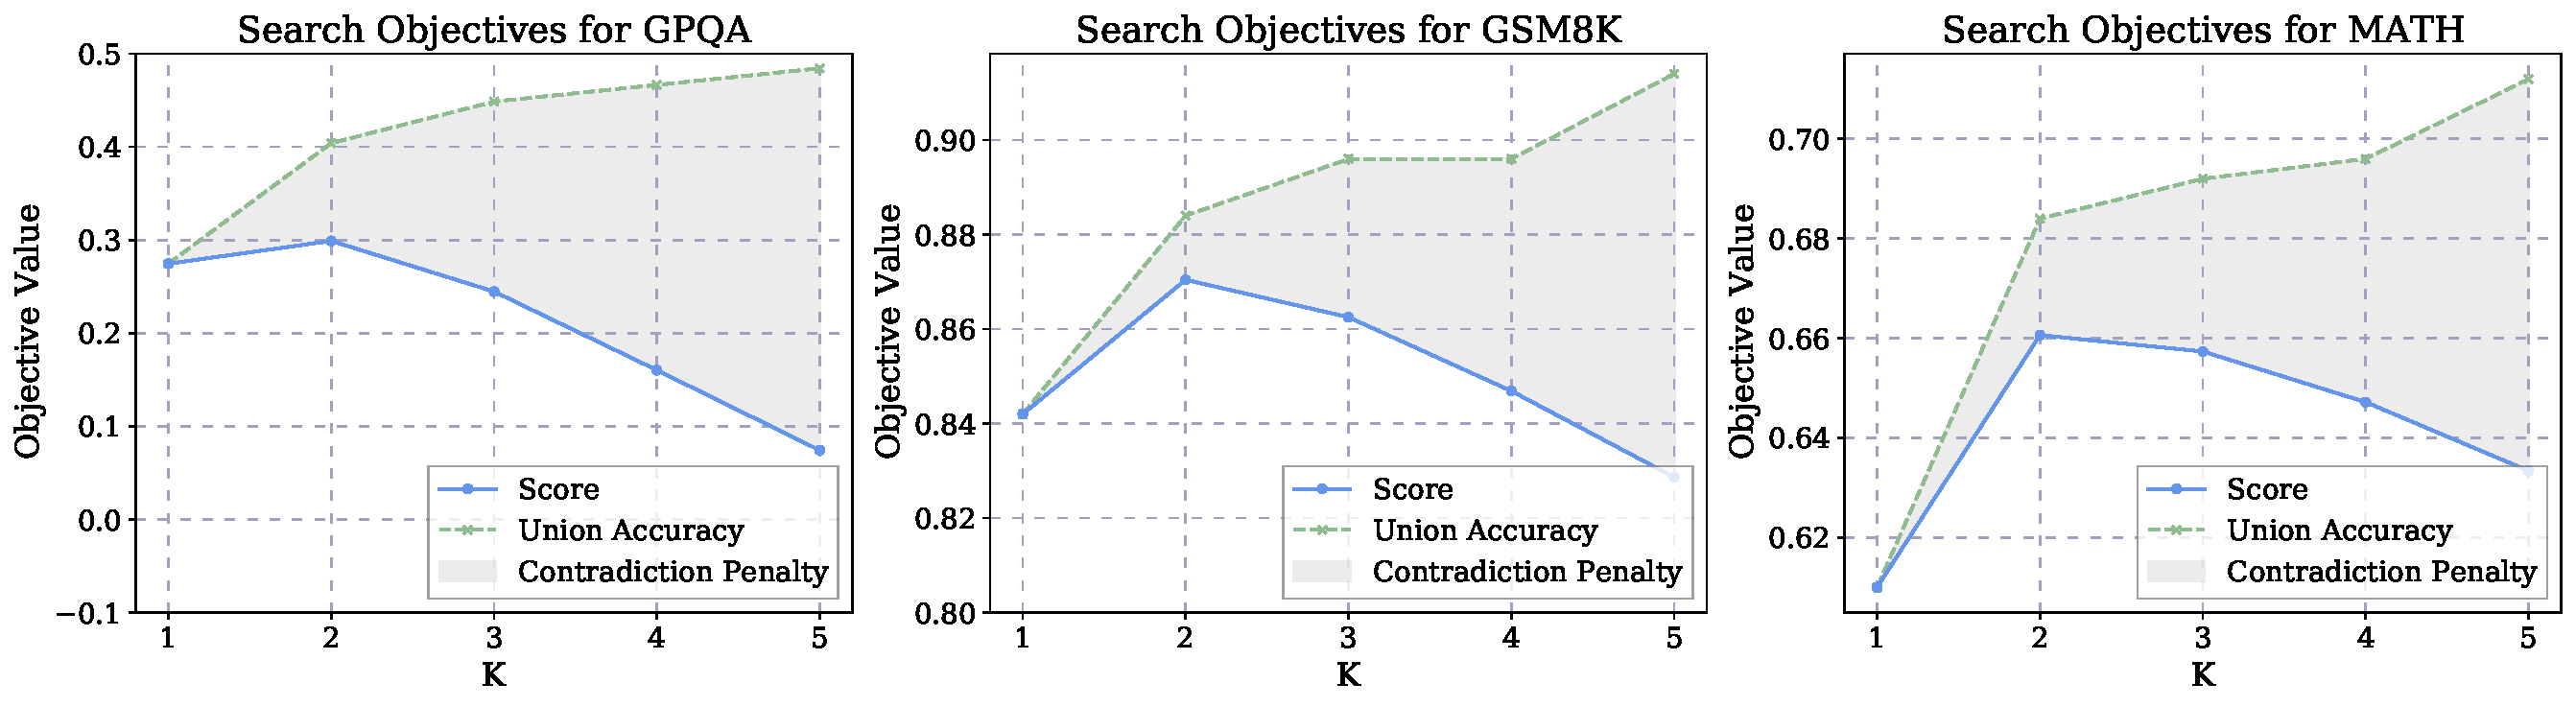
\includegraphics[width=\textwidth]{Figures/search_summary_comparison.pdf}
    \vspace{-20pt}
    \caption{\textbf{Union Accuracy and Contradiction Penalty both Increases as more models are added}. We plot the search objectives as the number of models (K) increases from 2 to 5 across three benchmarks. The green line denotes the union accuracy across models, the grey area indicates the contradiction penalty, and the blue line represents the overall search objective score. }
    % \vspace{-5pt}
    \label{fig:search_objectives}
\end{figure}


% \paragraph{Discussion \& Takeaways}
% Our results highlight two key takeaways. 
% First, model selection search is crucial for unlocking the potential of the \NAME{}. As shown in Table~\ref{tab:composition-combined}, naively combining three models without search provides little improvement over the single best model on the GPQA benchmark. In sharp contrast, our search-based method identifies a two-model orchestration that boosts accuracy by 4.4\% (Table~\ref{tab:final_results}), demonstrating the clear value of our approach.

% Second, the search process addresses a trade-off. Figure~\ref{fig:search_objectives} illustrates that as the number of models ($K$) in a orchestration increases, the union accuracy also increases. However, this is counterbalanced by a rise in the contradiction penalty, which indicates a higher frequency of conflicting predictions. This suggests that an effective model orchestration is determined by achieving a favorable balance between the union accuracy and contradiction.

\looseness=-1
To examine whether model selection search benefits \NAME{}, we construct a validation set of 500 questions sampled from the training splits of MATH, GPQA, and GSM8K. The candidate pool consists of five SLMs: Gemma 2 27B, Llama 3.1 8B, Mistral Small 24B~\citep{mistral_small_24b_instruct}, Mixtral 8$\times$7B, and Qwen2.5 7B~\citep{qwen2025qwen25technicalreport}. For each question, we collect three independent generations per model with temperature 0.5, repeating this process three times to obtain stable accuracy estimates.
The search procedure considers orchestrations with $K=2$ to $5$ models and is guided by an objective function mentioned in Section~\ref{sect:method}, with hyperparameter $\lambda=1$. The behavior of this objective is illustrated in Figure~\ref{fig:search_objectives}, showing the trade-off as $K$ increases. For simplicity, we select two representative two-model combinations from the search results for evaluation on the test set.

\paragraph{Results} Table~\ref{tab:composition_results_combined} summarizes the outcome of the search. The table lists the top-performing two-model combinations identified on the validation set, along with their evaluation on the held-out test set. Across benchmarks, these optimized orchestrations yield consistent improvements over the strongest individual models: accuracy increases by 4.5\% on MATH, 4.4\% on GPQA, and 4.3\% on GSM8K. This contrasts with Section~\ref{sub:vanilla}, where naive three-model combinations provide little to no benefit on GPQA. Figure~\ref{fig:search_objectives} further illustrates the underlying trade-off: while union accuracy rises with additional models, the contradiction penalty also grows, emphasizing that effective orchestration requires balancing these competing factors rather than simply enlarging the orchestration size.



% \begin{table}[hbtp]
% \centering
% \small


% \begin{tabular}{lll}
% \toprule
% \textbf{Dataset} & \textbf{Group 1} & \textbf{Group 2} \\
% \midrule
% \textbf{MATH}    & \makecell[l]{Mistral Small 24B \\ Qwen2.5 7B}         & \makecell[l]{ Qwen2.5 7B \\ Llama 3.1 8B} \\
% \midrule % 
% \textbf{GPQA}    & \makecell[l]{Gemma 2 27B \\ Mistral Small 24B}        & \makecell[l]{Llama 3.1 8B \\ Mistral Small 24B} \\
% \midrule % 
% \textbf{GSM8K}   & \makecell[l]{Mistral Small 24B \\ Qwen2.5 7B}         & \makecell[l]{Llama 3.1 8B \\ Mixtral 8x7B } \\
% % \midrule % 
% % \textbf{MMLU}    & \makecell[l]{Qwen 2.5 7B \\ Mistral Small 24B}        & \makecell[l]{Mistral Small 24B \\ Llama 3.1 8B} \\
% \bottomrule
% \end{tabular}
% \vspace{-5pt}
% \caption{\small \textbf{Model Combination Search Results} We show two top groups of models per dataset.}
% \label{tab:SLM-Mux-model-search-candidates-ruled}
% % \vspace{-15pt}
% \end{table}



% \begin{table*}[hbtp]
% \centering
% \begin{tabular}{l@{\hspace{3em}}ccc@{\hspace{3em}}ccc}
% \toprule
% \multirow{2}{*}{\textbf{Benchmark}} & \multicolumn{3}{c}{\textbf{Group 1}} & \multicolumn{3}{c}{\textbf{Group 2}} \\
% \cmidrule(lr){2-4} \cmidrule(lr){5-7}
% & \begin{tabular}[c]{@{}c@{}}Best Single\\ (Acc. \%)\end{tabular} & \begin{tabular}[c]{@{}c@{}}Composed\\ (Acc. \%)\end{tabular} & \begin{tabular}[c]{@{}c@{}}$\Delta$\\ (Gain)\end{tabular} & \begin{tabular}[c]{@{}c@{}}Best Single\\ (Acc. \%)\end{tabular} & \begin{tabular}[c]{@{}c@{}}Composed\\ (Acc. \%)\end{tabular} & \begin{tabular}[c]{@{}c@{}}$\Delta$\\ (Gain)\end{tabular} \\
% \midrule
% MATH & $75.5 \pm 1.5$ & $80.0 \pm 0.7$ & $+4.5$ & $75.5 \pm 1.5$ & $77.7 \pm 0.7$ & $+2.2$ \\
% GPQA & $45.1  \pm  2.8$ & $49.5  \pm  1.8$ & $+4.4$ & $45.1  \pm  2.8$ & $48.8  \pm  0.8$ & $+3.6$ \\
% GSM8K & $88.5 \pm 0.7$ & $92.8 \pm 0.6$ & $+4.3$ & $80.8 \pm 2.1$ & 
% $85.2 \pm 0.7$& $+4.4$ \\
% % MMLU & $77.2 \pm 0.8$ &  $74.5 \pm 0.8$ & $-2.7$ & $77.2 \pm 0.8$ & $73.4 \pm 0.7$ & $-3.8$ \\
% \bottomrule

% \end{tabular}
% \vspace{-5pt}
% \caption{\small \textbf{Evaluation Results of Selected Models} Composed Acc shows the accuracy of groups 1 \& 2 on the test set using the \NAME{}. Best Single is the accuracy of the best individual model in the orchestration. Gain indicates the improvement over the best single accuracy. }
% \label{tab:final_results}
% \vspace{-10pt}
% \end{table*}


\begin{table*}[t]
\centering
\setlength{\tabcolsep}{18pt}
\renewcommand{\arraystretch}{0.9}
\resizebox{\textwidth}{!}{
\small
% Using 'c' for the numeric columns to ensure they are centered.
\begin{tabular}{l c l c c c}
\toprule
\textbf{Benchmark} & \textbf{Group} & \textbf{Model Selection} & \begin{tabular}[c]{@{}c@{}}\textbf{Best Single}\\ \textbf{(Acc. \%)}\end{tabular} & \begin{tabular}[c]{@{}c@{}}\textbf{Composed}\\ \textbf{(Acc. \%)}\end{tabular} & \begin{tabular}[c]{@{}c@{}}\textbf{$\Delta$}\\ \textbf{(Gain)}\end{tabular} \\
\midrule
\textbf{MATH} & 1 & \makecell[l]{Mistral Small 24B \\ Qwen2.5 7B} & $75.5 \pm 1.5$ & $80.0 \pm 0.7$ & $+4.5$ \\
\cmidrule(l){2-6}
              & 2 & \makecell[l]{Qwen2.5 7B \\ Llama 3.1 8B} & $75.5 \pm 1.5$ & $77.7 \pm 0.7$ & $+2.2$ \\
\midrule
\textbf{GPQA} & 1 & \makecell[l]{Gemma 2 27B \\ Mistral Small 24B} & $45.1 \pm 2.8$ & $49.5 \pm 1.8$ & $+4.4$ \\
\cmidrule(l){2-6}
              & 2 & \makecell[l]{Llama 3.1 8B \\ Mistral Small 24B} & $45.1 \pm 2.8$ & $48.8 \pm 0.8$ & $+3.6$ \\
\midrule
\textbf{GSM8K} & 1 & \makecell[l]{Mistral Small 24B \\ Qwen2.5 7B} & $88.5 \pm 0.7$ & $92.8 \pm 0.6$ & $+4.3$ \\
\cmidrule(l){2-6}
               & 2 & \makecell[l]{Llama 3.1 8B \\ Mixtral 8$\times$7B} & $80.8 \pm 2.1$ & $85.2 \pm 0.7$ & $+4.4$ \\
\bottomrule
\end{tabular}
}
\vspace{-5pt}
\caption{\small \textbf{Model Selection Search and Evaluation Results.} We show the top two model groups identified by our search for each benchmark. For each group, we report the accuracy of the best-performing single model within the orchestration, the accuracy achieved by our \NAME{}, and the resulting performance gain.}
\label{tab:composition_results_combined}
\vspace{-8pt}
\end{table*}

% \vspace{-5pt}
\vspace{3pt}
\subsection{Compute Scaling Strategies Reveal Optimal Resource Allocation}
\vspace{3pt}

% \vspace{-3pt}
\label{sub:scaling-results}
% We  examine two dimension of compute scaling as mentioned in Section~\ref{sec:scaling}. For the ``Adding More Participating Model Types'' dimension, we run this experiment by searching for the best orchestration under budget from 2 to 5 and then evaluate them. We conduct the experiment on the validation set. We report the mean accuracy in Figure~\ref{fig:scaling_model_counts}. 

To evaluate the ``Adding More Participating Model Types" dimension of compute scaling, we assess how performance changes as the number of models in the orchestration increases. For each number of models from 2 to 5, we first apply the search method from Section~\ref{sub:method-search} to identify the optimal model selection from our pool. We then evaluate \NAME{} with selected models on the validation set. Figure~\ref{fig:scaling_model_counts} plots the resulting mean accuracy (blue line, left y-axis) for each value of K. To illustrate the theoretical performance ceiling of each ensemble, we also plot the union accuracy (grey line, right y-axis), defined as the percentage of questions solved by at least one model in the group.


\begin{table}[h]
\centering
\setlength{\tabcolsep}{20pt}
\renewcommand{\arraystretch}{0.9}
\resizebox{\textwidth}{!}{
\small
\begin{tabular}{l c c c c}
\toprule
\textbf{Benchmark} & \textbf{Samples} & \textbf{\NAME{}} & \textbf{Agent Forest} & \textbf{$\Delta$ (Gain)} \\
\midrule
\multirow{2}{*}{MATH} & 2 & $76.8 \pm 0.7$ & $72.3 \pm 1.5$ & +4.5 \\
& Best & $79.5 \pm 0.4$ & $79.2 \pm 0.4$ & +0.3 \\
\midrule
\multirow{2}{*}{GPQA} & 2 & $46.3 \pm 2.3$ & $40.4 \pm 2.3$ & +5.9 \\
& Best & $48.8 \pm 1.2$ & $47.6 \pm 1.4$ & +1.2 \\
\midrule
\multirow{2}{*}{GSM8K} & 2 & $82.1 \pm 0.7$ & $77.7 \pm 0.2$ & +4.4 \\
& Best & $86.5 \pm 0.8$ & $84.3 \pm 0.8$ & +2.2 \\
\bottomrule
\end{tabular}
}
\vspace{-5pt}
\caption{\textbf{Comparison of \NAME{} and Agent Forest.} We compare \NAME{} and Agent Forest in two settings: \textbf{(1)} with 2 samples per model (Samples=2), and \textbf{(2)} using the best accuracy found during scaling for each method (Samples=best). In the second setting, the number of samples per model may vary. }
% \vspace{-5pt}
\label{tab:SLM-Mux_vs_af_comparison}
\end{table}


For the ``Drawing More Samples per Model'' dimension, we reuse the two groups of models listed in Table~\ref{tab:composition_results_combined}. We vary the number of samples per model from 2 to 9 and report the mean accuracy of \NAME{} over three runs for each sample budget. The results are presented in Figure~\ref{fig:samples_per_model}, along with a baseline, Agent Forest~\citep{li2024agentsneed}, for comparison. To ensure fairness, Agent Forest is reproduced using the same models from Group 2. We report the best accuracy achieved by the \NAME{} when scaling with Samples per Model and compare it to the accuracy of the single best model in the orchestration, as shown in Table~\ref{tab:composition_results_combined}. 



\paragraph{Results} The effect of ``Adding More Participating Model Types'' varies substantially across benchmarks. On GPQA, accuracy peaks when combining two models and declines thereafter. On GSM8K, accuracy quickly saturates at two models without further gains. In contrast, on MATH, accuracy continues to improve as additional models are included. Despite these differences, the union accuracy of model orchestration consistently increases with more models, emphasizing the role of output contradictions among models, as elaborated in Section~\ref{sub:method-search}.

``Drawing More Samples per Model'' yields more consistent improvements across benchmarks. Moreover, under this setting, our \NAME{} systematically outperforms Agent Forest, with the largest margin observed on GPQA, where single-model accuracy is lowest. 

% \subsection{Head to head comparison with other methods}

% \paragraph{Results}: we compare our \NAME{}

% Table~\ref{tab:SLM-Mux_vs_af_comparison} further provides a quantitative comparison with Agent Forest. 

\begin{figure}[t]
    \centering
    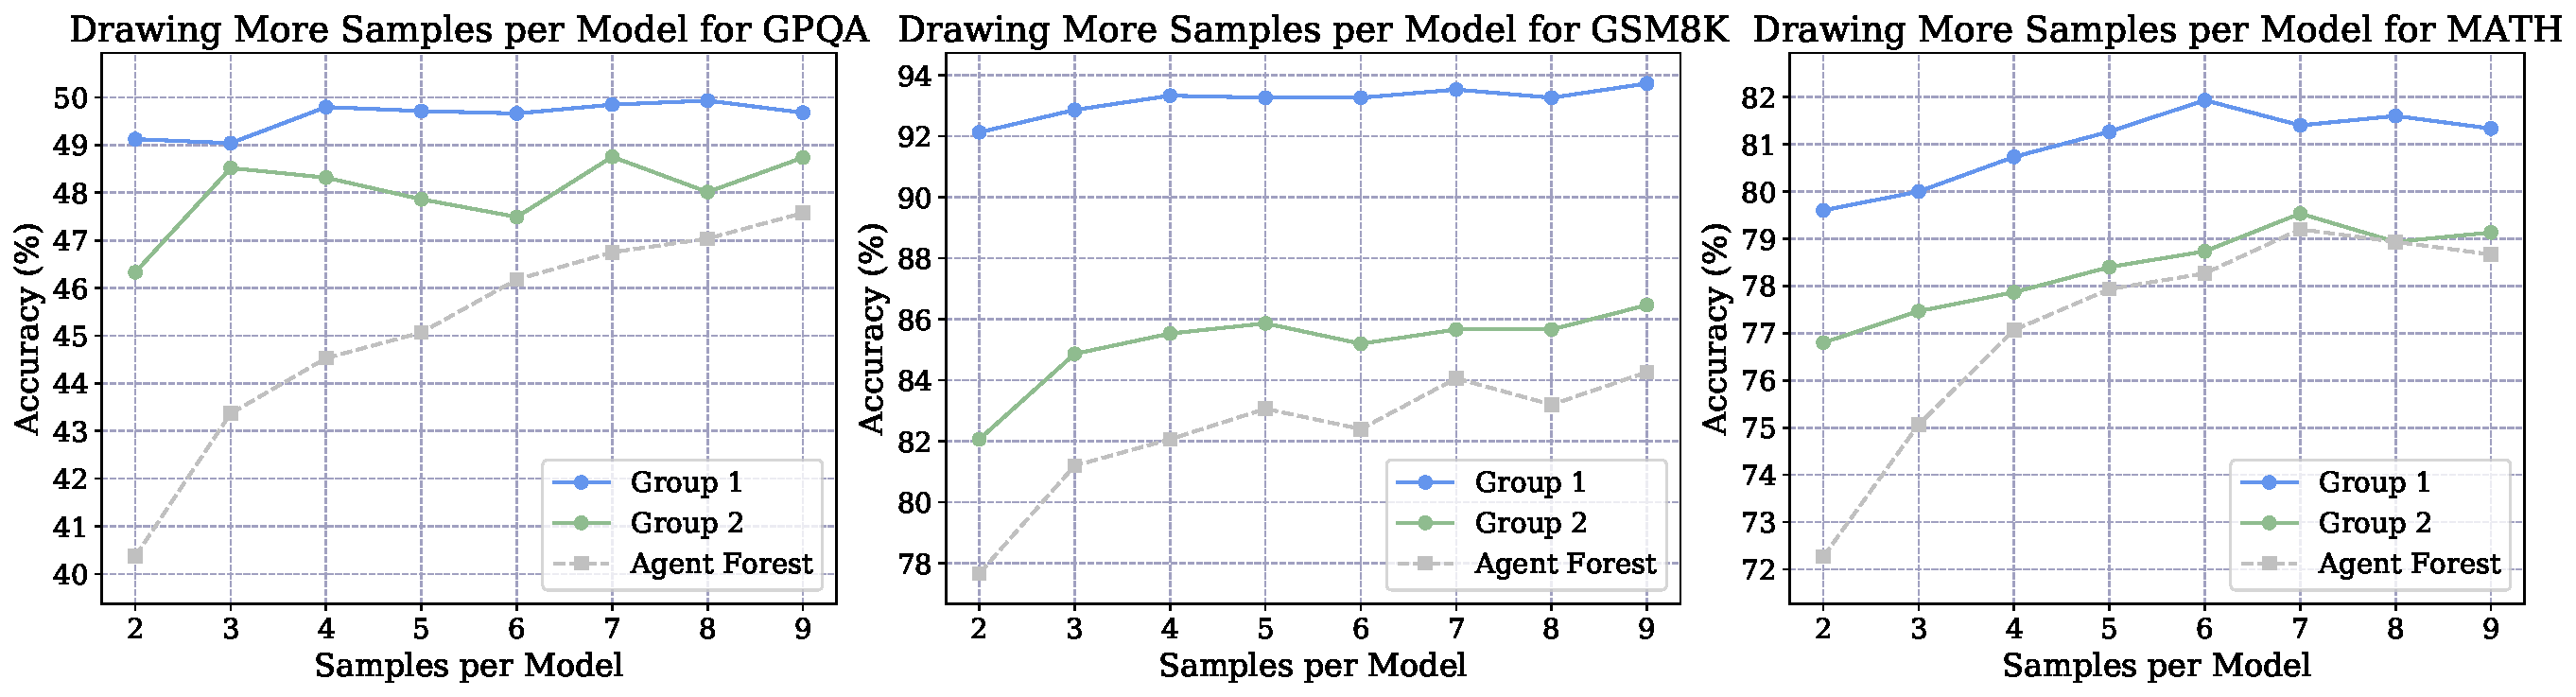
\includegraphics[width=\textwidth]{Figures/scaling_curves.pdf}
    \vspace{-20pt}
    \caption{\small \textbf{Drawing More Samples per Model Improves Accuracy}. We report mean accuracy of \NAME{} as the number of samples per model increases from 2 to 9 across three benchmarks. Group 1 and Group 2 are from  Table~\ref{tab:composition_results_combined}. We also plotted the mean accuracy of Agent Forest~\citep{li2024agentsneed} in grey line. }
    \vspace{-15pt}
    \label{fig:samples_per_model}
\end{figure}

\begin{figure}[t]
    \centering
    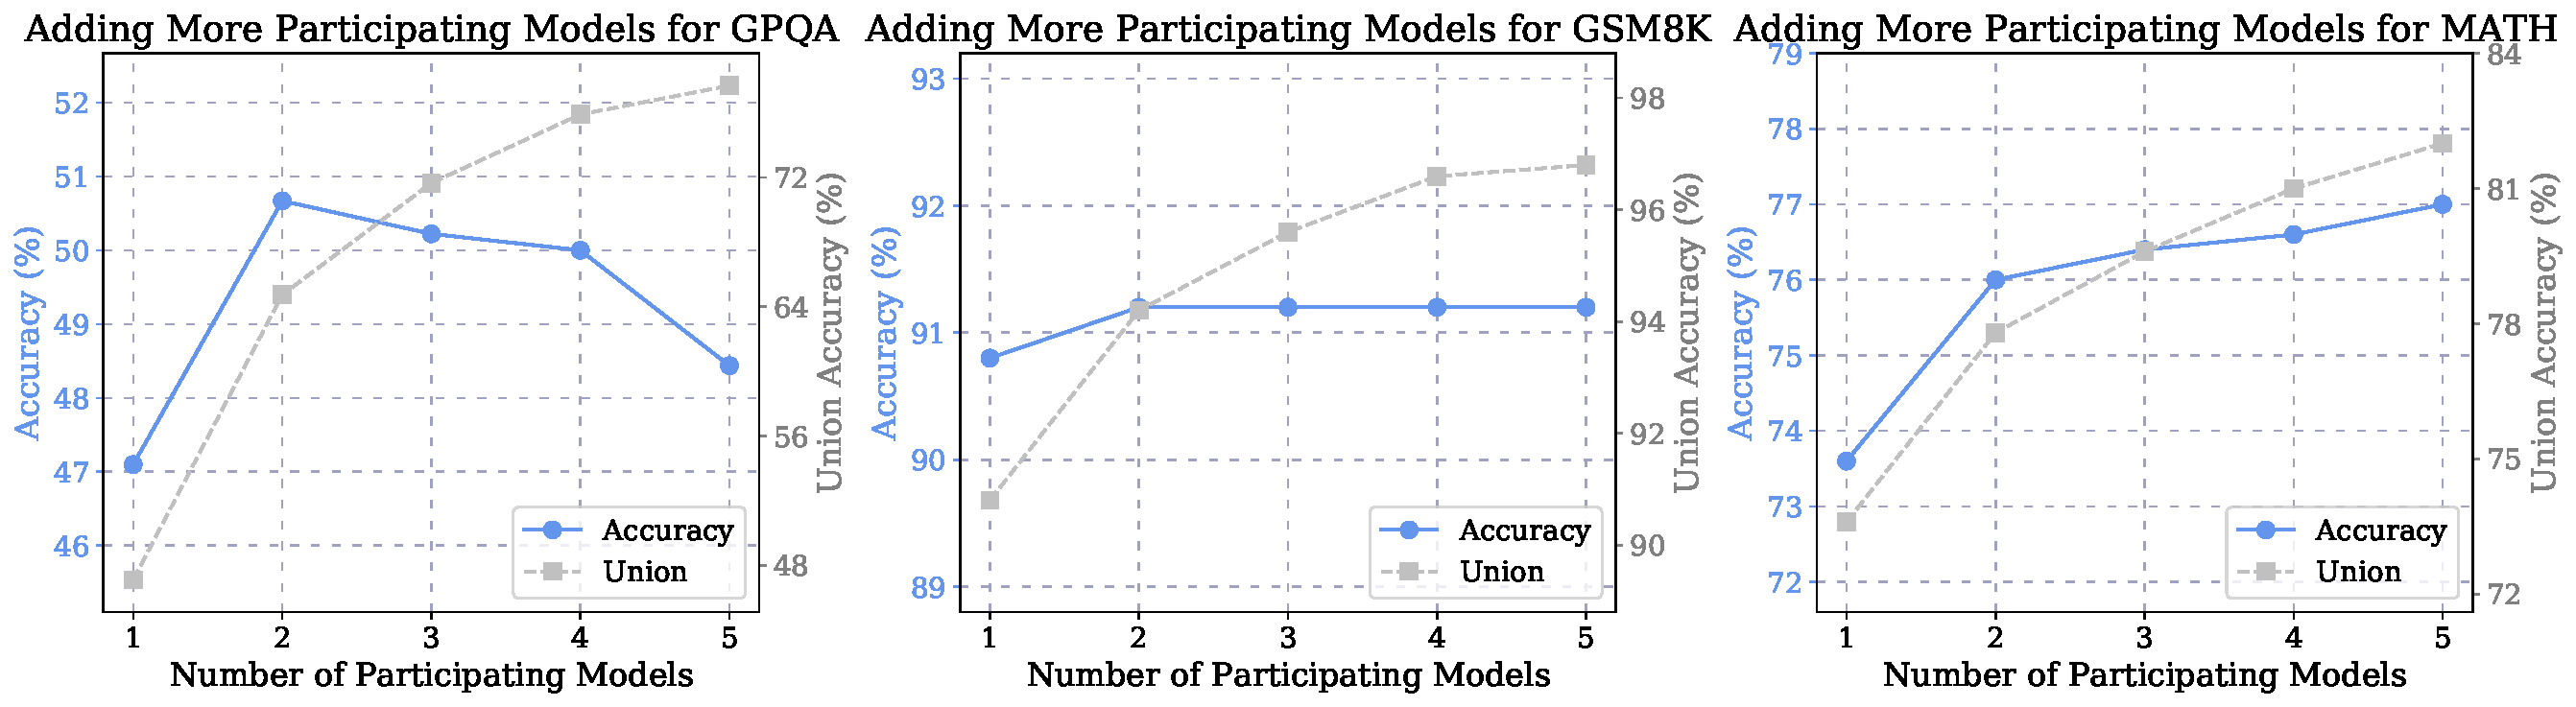
\includegraphics[width=\textwidth]{Figures/Adding_More_Participating_Models.pdf}
    \vspace{-20pt}
    \caption{\small \textbf{Adding More Participating Models Affects Accuracy Differently}. We report the mean accuracy (blue line) of the optimal \NAME{}  obtained when using 2 to 5 models across three benchmarks. We also report the union accuracy (grey line), defined in Section~\ref{sub:method-search}. The blue line (Mean Accuracy) is plotted against the left-hand Y-axis. The grey line (Union Accuracy) is plotted against the right-hand Y-axis. }
    % \vspace{-5pt}
    \label{fig:scaling_model_counts}
\end{figure}

% \begin{table}[htbp]
% \centering

% \small
% \begin{tabular}{l@{\hspace{2em}}cc@{\hspace{2em}}cc}
% \toprule
% \multirow{2}{*}{\textbf{Benchmark}} & \multicolumn{2}{c}{\textbf{Group 1}} & \multicolumn{2}{c}{\textbf{Group 2}} \\
% \cmidrule(lr){2-3} \cmidrule(lr){4-5}
% & \begin{tabular}[c]{@{}c@{}}Acc. \% \end{tabular} & \begin{tabular}[c]{@{}c@{}}$\Delta$ (Gain)\end{tabular} & \begin{tabular}[c]{@{}c@{}}Acc. \% \end{tabular} & \begin{tabular}[c]{@{}c@{}}$\Delta$ (Gain)\end{tabular} \\
% \midrule
% MATH & $81.9 \pm 0.2$ & $+6.4$ & $79.5 \pm 0.4$ & $+4.0$ \\
% GPQA & $49.9 \pm 1.8$ & $+4.8$ & $48.7 \pm 1.2$ & $+3.6$ \\
% GSM8K & $93.7 \pm 0.2$ & $+5.2$ & $86.5 \pm 0.8$ & $+5.7$ \\
% \bottomrule

% \end{tabular}
% \caption{\textbf{Best Accuracy after Sample Scaling} Acc indicates the highest accuracy achieved through scaling. Groups 1 \& 2 are defined in Table~\ref{tab:composition_results_combined}. Gain represents the improvement over the best single-model accuracy reported in Table~\ref{tab:composition_results_combined}.}
% \label{tab:scaling_best}
% \end{table}


\begin{table}[h]
\centering
\vspace{-10pt}
\setlength{\tabcolsep}{15pt}
\renewcommand{\arraystretch}{1.0}
\resizebox{\textwidth}{!}{
\small
\begin{tabular}{l@{\hspace{2em}}cc@{\hspace{2em}}cc@{\hspace{2em}}c}
\toprule
\multirow{2}{*}{\textbf{Benchmark}} & \multicolumn{2}{c}{\textbf{Group 1}} & \multicolumn{2}{c}{\textbf{Group 2}} & \multirow{2}{*}{\textbf{Qwen-2.5 72B Acc. \%}} \\
\cmidrule(lr){2-3} \cmidrule(lr){4-5}
& Acc. \% & $\Delta$ (Gain) & Acc. \% & $\Delta$ (Gain) &  \\
\midrule
MATH  & $81.9 \pm 0.2$ & $+6.4$ & $79.5 \pm 0.4$ & $+4.0$ & $82.3 \pm 0.5$ \\
GPQA  & $49.9 \pm 1.8$ & $+4.8$ & $48.7 \pm 1.2$ & $+3.6$ & $44.9 \pm 0.5$ \\
GSM8K & $93.7 \pm 0.2$ & $+5.2$ & $86.5 \pm 0.8$ & $+5.7$ & $90.4 \pm 0.3 $ \\
\bottomrule
\end{tabular}
}
\vspace{-5pt}
\caption{\textbf{Best Accuracy after Sample Scaling beats Larger Model.} 
Acc indicates the highest accuracy achieved through scaling. 
Groups 1 \& 2 are defined in Table~\ref{tab:composition_results_combined}. 
Gain represents the improvement over the best single-model accuracy reported in Table~\ref{tab:composition_results_combined}. 
For reference, we also include the performance of the large model Qwen-2.5 72B, showing that our composed small models can outperform it on GPQA and GSM8K.}
\label{tab:scaling_vs_qwen}
\vspace{-10pt
}
\end{table}



% \begin{table}[t]
% \centering
% \caption{Accuracy (\%) of different models on sampled questions from MATH, MMLU, GPQA, and GSM8K. 
% Each result is averaged over 3 runs (temperature = 0.5).\cw{This table should be put into appendix.}}
% \label{tab:exp_results}
% \resizebox{\textwidth}{!}{
% \begin{tabular}{lccccccc}
% \toprule
% Dataset & Gemma 2 27B & Qwen2.5-3B & Llama 3.2 3B & Llama 3.1 8B & Mistral Small 24B & Mixtral 8$\times$7B v0.1 & Qwen2.5-7B \\
% \midrule
% MATH   & $62.0 \pm 0.0$ & $51.0 \pm 2.0$ & $51.3 \pm 2.1$ & $50.3 \pm 1.5$ & $70.0 \pm 2.6$ & $34.0 \pm 3.5$ & $74.0 \pm 2.6$ \\
% MMLU   & $76.7 \pm 0.6$ & $35.0 \pm 5.6$ & $53.0 \pm 1.0$ & $57.3 \pm 2.1$ & $72.3 \pm 1.2$ & $62.3 \pm 1.5$ & $71.0 \pm 1.0$ \\
% GPQA   &  --  &  --  &  --  &  --  &  --  &  --  &  --  \\
% GSM8K  &  --  &  --  &  --  &  --  &  --  &  --  &  --  \\
% \midrule
% Average &  --  &  --  &  --  &  --  &  --  &  --  &  --  \\
% \bottomrule
% \end{tabular}
% }
% \label{tab:search_single_acc}
% \end{table}

% \subsection{Heterogeneous Instruction Tuning}

% \begin{table}[t]
%   \centering
%   \footnotesize
  
 
%   \begin{tabular}{lrrrr}
%     \toprule
%     \textbf{Method} & \textbf{Acc (\%)} & \textbf{$\Delta$ Acc (\%)} &
%     \textbf{Token Usage} & \textbf{$\Delta$ Tokens (\%)} \\
%     \midrule
%     Mixture-of-Agents                   & 58.6 & --   &   720,843  & --    \\
%     Mixture-of-Agents (w/ \NAME{})          & 59.6 & +1.0 &   595,269  & -17.4 \\
%     \midrule
%     LLM-Debate                          & 65.6 & --   & 1,960,680  & --    \\
%     LLM-Debate (w/ \NAME{})                 & 61.1 & -4.5 &   786,841  & -59.9 \\
%     \midrule
%     Multi-Agent Verification            & 64.2 & --   & 5,318,019  & --    \\
%     Multi-Agent Verification (w/ \NAME{})   & 61.6 & -2.6 & 1,249,373  & -76.5 \\
%     \midrule
%     \NAME{} (k=1)                           & 60.6 & --   &   581,498  & --    \\
%     \NAME{} (k=3)                           & \textbf{68.2} & --   & 1,509,557  & --    \\
%     \midrule
%     Upper Bound                         & 78.3 & --   &   --  & --    \\
%     \bottomrule
%   \end{tabular}
%   \vspace{5pt}
%   \caption{\small \textbf{\NAME{} Improves Computational Efficiency on GPQA.} Performance and computational efficiency of compositional methods on the GPQA dataset. 
%            "$\Delta$ Acc (\%)" indicates the accuracy difference achieved by the \NAME{} variant compared to
%            the original method, and "$\Delta$ Tokens (\%)" gives the relative token-usage reduction.}
%     \label{tab:composition-gpqa}
%     \vspace{-10pt}
% \end{table}
% % \vspace{-10pt}





